\pagestyle{fancy}
\renewcommand{\theUnit}{8}
\ifthenelse{\isundefined{\UnitPageNumbers}}{}{\setcounter{page}{1}}
\rhead{Chapter  \theUnit: Hypothesis Tests}
\lhead{Math 3382: Statistical Theory}
%\lhead{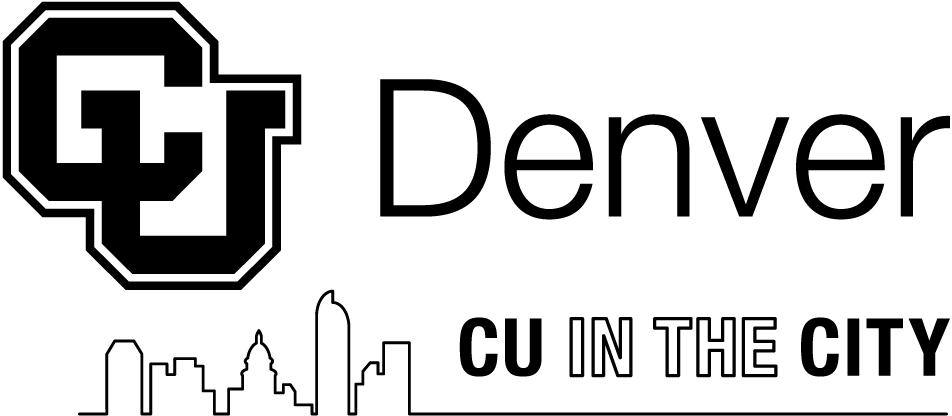
\includegraphics[width=1.25cm]{CUDenver-Logo.png}}
\rfoot{\mypage}
\cfoot{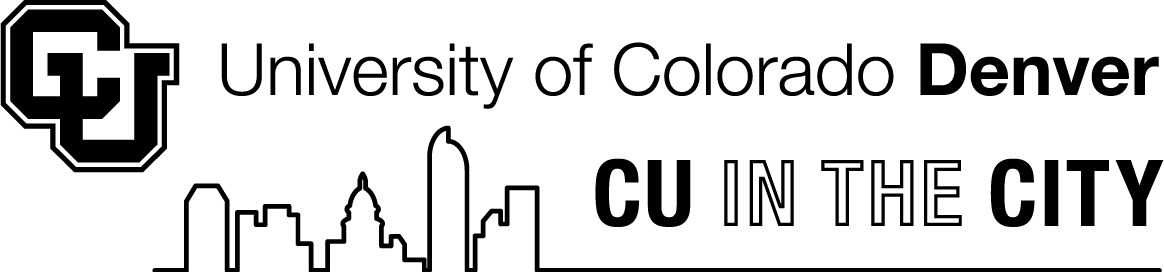
\includegraphics[width=2.25cm]{CUDenver-Logo-coverpage.png}}
\lfoot{Adam Spiegler}
\fancypagestyle{firstfooter}{\footskip = 50pt}
\renewcommand{\footrulewidth}{.4pt}
%%%%%%%%%%%%%%%%%%%%%%%%%%%
\vspace*{-20pt} \thispagestyle{firstfooter}


%\begin{tasks}[counter-format = {(tsk[a])},label-offset = {0.8em},label-format = {\color{black}\bfseries}](2)
\pagebegin{Section 8.3: Hypothesis Tests For Means and Proportions: Two Populations}


\bb
\ii State whether each set of hypotheses is valid for a statistical test.  If not, explain why not.  If so, would you use a one-tail or two-tail test.

\bb
\ii $H_0:  \mu = 50$ and $H_a: \mu > 50$. \ms
\ii $H_0: p_a - p_b <0$ and $H_a:  p_a - p_b=0$. \ms
\ii $H_0:  \mu_1 - \mu_2 \ne 0 $ and $H_a: \mu_1 -\mu_2 =0$. \ms
\ii $H_0:  p_a = p_b$ and $H_a: p_a \ne p_b$. \ms
\ii $H_0: \bar{x} = 5$ and $H_a:  \bar{x} \ne 5$. \ms
\ii $H_0: p = 0.25$ and $H_a: p>0.5$. \ms
\ii $H_0: p = 0.25$ and $H_a: p>0.25$. \ms
\ii $H_0: \mu = 10$ and $H_a:  \mu \ne 10$. \ms
\ee


\ii Reflect on the previous question, and list some key points to keep in mind when stating hypotheses.

\vfill
\ee


\clearpage

\pagebegin{Hypothesis Test For a Difference in Two Means }

\bbox
Let $X_1, X_2, \ldots , X_{n_1} \sim N(\mu_1, \sigma_1^2)$  and $Y_1, Y_2, \ldots , Y_{n_2} \sim N(\mu_2, \sigma_2^2)$ be a random samples from two independent normal populations  with sample means and standard deviations $\bar{X}$, $S_1$ and $\bar{Y}$, $S_2$, respectively. To test for a difference between the two means we form the test statistic:
\colorb{\[ t = \frac{\bar{X}-\bar{Y}}{\sqrt{\frac{S_1^2}{n_1}+ \frac{S_2^2}{n_2}}}.\]}
To compute the P-value:
\bi
\ii Use a $t$-distribution with degrees of freedom computed by Welch's approximation.
\ii  \textbf{\colorb{t.test(Variable1 $\sim$ HowGroupsSplit, data = Dataset\_name, alt = ``greater'')}}.
\ii Use ``greater'' for right-tail test, ``less'' for left-tail test. No alt option does a two-tail test.
\ii When doing the calculation by hand, we can use $d.\!f.\! = n_{\rm min} -1$.
\ei
\ebox

\bb[resume]
\ii A researcher suggests that male nurses earn more than female nurses. A survey of 16 male nurses and 20 female nurses reports these data. The mean salary for the 20  females is \$$23,\!750$ with a standard deviation of \$$250$.  The mean salary for the 16  males is \$$23,\!900$ with a standard deviation of \$$300$. Is there enough evidence to support the claim that female nurses earn less than male nurses? Use $\alpha=0.05$.

\medskip

\bb
\ii State the hypotheses. \vspace{0.6in}
\ii Compute the test value and P-value by hand. \vfill
\ii Make a decision and summarize the results.\vspace{1.5in}
\ee
\ee

\clearpage
\pagebegin{Hypothesis Test For a Difference in Two Proportions}


\bbox
Let $X_1 \sim \mbox{Binom}(n_1, p_1)$ and $X_2 \sim \mbox{Binom}(n_2, p_2)$ be two independent random variables. To test for the difference in two proportions we form the test statistic:
\colorb{\[ z= \frac{\hat{p}_1-\hat{p}_2}{\sqrt{\hat{p}_p(1-\hat{p}_p) \left( \frac{1}{n_1}+\frac{1}{n_2} \right) }},\]}
where \textbf{\colorr{$\hat{p}_p = (X_1+X_2)/(n_1+n_2)$ is the pooled proportion}}.
To compute the P-value:
\bi
\ii Use a normal distribution.
\ii \textbf{\colorb{prop.test(c($x_1$, $x_2$), c($n_1$, $n_2$), alt = ``blah'')}}
\ei
\ebox

 \bb[resume]
 \ii It is believed that a sweetener called xylitol helps prevent ear infections. In a randomized experiment $n_1 = 165$ children took a placebo and $68$ of them got ear infections. Another $n_2 = 159$ children took xylitol and $46$ of them got ear infections. We believe that the proportion of ear infections in the placebo group will be greater than the xylitol group. Use $\alpha=0 .01$.

\bb
\ii State the hypotheses. \vspace{0.6in}
\ii Compute the test value and P-value by hand. \vfill
\ii Enter R code to calculate the test statistic and P-value.\vspace{0.6in}
\ii Make a decision and summarize the results. \vspace{1.5in}
\ee
\ee

%\ii \textbf{Be nice to pigeons?} In a study\footnote{Belguermi, A., ``Pigeons discriminate between human feeders,'' \textit{Animal Cognition}, 2011} conducted in Paris, equal amounts of pigeon feed were spread on the ground in two adjacent locations. One person was assigned to be ``hostile'' and the other person ``nice''.  The two people were randomly exchanged between the two locations throughout the study. It seemed that the pigeons learned to avoid the hostile person's location.

\clearpage

 \bbox   
  \bi
  \ii Binomial distributions are discrete, but the CLT approximation uses a normal distribution which is continuous.
  '\ii We can improve the approximation using a \alert{continuity correction} (see Chapter 4).
  \ii Add or subtract $0.5$ from each ``success'' count so the \alert{difference in proportions becomes closer to 0}, and thus gives a larger P-value.
  \ei
\ebox

\bb[resume]
\ii It is believed that a sweetener called xylitol helps prevent ear infections. In a randomized experiment $n_1 = 165$ children took a placebo and $68$ of them got ear infections. Another $n_2 = 159$ children took xylitol and $46$ of them got ear infections. We believe that the xylitol will reduce the incidence of ear infections when compared to no treatment. Use $\alpha=0 .01$. \bigskip

Compute the test value and P-value by hand.
\ee

\clearpage


\bb[resume]
\ii In the \textit{NCBirths2004} dataset, the variable Weight gives the weight in grams of a random sample of 1009 newborns in North Caroline in 2004. The variable Tobacco indicates whether the birth mother is a smoker or not. Researchers want to determine whether mean weight of all babies born North Carolina in 2004 to nonsmoking mothers is different from the mean of all babies born from mothers that are smokers?
\bb
\ii Set up the hypotheses.  \vspace{1in}
\ii Using R calculate the test statistic and P-value. \vspace{1.5in}
\ii Summarize the test results.  \vspace{1.5in}
\ee


\clearpage
\pagebegin{Test Your Own Claims!}

\ii The dataset \textit{NCBirths2004} has the following variables:
\bi
\ii MothersAge: Categorical variable (under 15, 15-19, 20-24, 25-29, 30-34, 35-39, 40-44, 45-49).
\ii Tobacco: Categorical (Yes or No)
\ii Alcohol: Categorical (Yes or No)
\ii Gender: Categorical (Male or Female) - Gender of assigned at birth to baby.
\ii Weight: Numerical (in grams)
\ii Gestation: Numerical (in weeks)
\ei

\bb
\ii Write one possible claim that could be tested by a hypothesis test for a difference in two means. Then write the corresponding hypotheses and R code you would use to calculate the P-value of the observed samples. \vfill
\ii Write one possible claim that could be tested by a hypothesis test for a difference in two proportions. Then write the corresponding hypotheses and R code you would use to calculate the P-value of the observed samples. \vfill
\ii Write one possible claim that could be tested by a hypothesis test for a in a single mean. Then write the corresponding hypotheses and R code you would use to calculate the P-value of the observed sample. \vfill
\ii Write one possible claim that could be tested by a hypothesis test for a single proportion. Then write the corresponding hypotheses and R code you would use to calculate the P-value of the observed sample. \vfill
\ee
\ee

\clearpage

\pagebegin{Section 8.3: Hypothesis Tests For Mean Difference in Matched Pairs}

\bb[resume]
\ii A study\footnote{de Lucas, Balidan, Neiva, Grecco, and Denadai. ``The effects of wetsuits on physiological and biomechanical indices during swimming'', \textit{Journal of Science and Medicine in Sport}} tested whether wearing wetsuits influences swimming velocity. Twelve competitive swimmers swam 1500 meters at maximum speed twice each. Once wearing a wetsuit and once wearing a regular bathing suit. The order of the trials was randomized. Each time, the maximum velocity in meters/sec of the swimmer was recorded.

\vspace{0.25in}

\begin{tabular}{|l||c|c|c|c|c|c|c|c|c|c|c|c|}
Swimmer & 1 & 2 & 3 & 4 & 5 & 6 & 7 & 8 & 9 & 10 & 11 & 12 \\
\hline
Wetsuit & $1.57$ & $1.47$ & $1.42$ & $1.35$ & $1.22$ & $1.75$ & $1.64$ & $1.57$ & $1.56$ & $1.53$ & $1.49$ & $1.51$ \\
No Wetsuit & $1.49$ & $1.37$ & $1.35$ & $1.27$ & $1.12$ & $1.64$ & $1.59$ & $1.52$ & $1.50$ & $1.45$ & $1.44$ & $1.41$ \\
\hline
Difference & $0.08$ &  $0.10$ &  $0.07$ &  $0.08$ &  $0.10$ & $0.11$ & $0.05$ & $0.05$ & $0.06$ & $0.08$ & $0.05$ &  $0.10$
\end{tabular}

\bb
\ii Set up the hypothesis for the test both in words and using appropriate notation. \vspace{0.6in}
\ii What do you think would be an appropriate test statistic we can use to gauge the significance of the sample?  \vfill 
\ii Calculate the P-value of the observed sample.  \vfill
\ii What would the conclusion  be at a 5\% significance level? Summarize the result in the context of this problem.  \vspace{0.5in}
\ee
\ee

